\documentclass{article}

\usepackage{url}
\usepackage{amsmath,amssymb}
\usepackage{graphicx,svg}

\begin{document}
\title{Lecture 5\\ Sampling and Reconstruction}
\author{C.L. Wyatt}
\date{\today}
\maketitle

Today's lecture is a review of material from ECE 2714. We will review sampling theory, the Nyquist rate, practical sampling, and reconstruction techniques.

Recall that hybrid systems are ones with both CT and DT signals. Such systems require the ability to:

\begin{itemize}
\item convert signals from CT to DT: sampling or analog-to-digital conversion (ADC)
\item convert signals from DT to CT: reconstruction or digital-to-analog conversion (DAC)
\end{itemize}

\section{Ideal Sampling Theory}

The impulse train

$$
x_p(t) = \sum\limits_{n = -\infty}^{\infty} \delta(t-nT)
$$

is a periodic function with period $T$. It has a CTFS representation

$$
x_p(t) = \sum\limits_{k = -\infty}^{\infty} a_k e^{j\frac{2\pi}{T} k t}
$$

where $a_k = \frac{1}{T}$ are the coefficients.

Its Fourier Transform is then

$$
X_p(j\omega) = \sum\limits_{k = -\infty}^{\infty} \delta\left(\omega-\frac{2\pi}{T} k\right)
$$

Given ans arbitrary signal $x(t)$ we can represent sampling as multiplication by the impulse train

$$
  x_s(t) = x(t)\cdot x_p(t)
  = \sum\limits_{n = -\infty}^{\infty} x(t)\cdot\delta(t-nT)
  = \sum\limits_{n = -\infty}^{\infty} x(nT)\cdot\delta(t-nT)
$$

where we define $x(nT) = x[n]$.

In the frequency domain, multiplication is convolution

$$
X_s(j\omega) = \frac{1}{2\pi} X_p(j\omega)*X(j\omega) = \frac{1}{T} \sum\limits_{n = -\infty}^{\infty} X\left(j\left(\omega - \frac{2\pi}{T} n \right) \right)
$$

The frequency content of the sampled signal consists of copies of the frequency content of the original signal called \textit{images}.

\section{Nyquist Criteria}

To ensure there is do distortion in the signal we require the images do not overlap, which occurs if $T < \frac{1}{2B}$, where $B$ is the \textit{bandwidth} of $x(t)$. This is the Nyquist criteria. In terms of a frequency this sample rate is then $\omega_0 = \tfrac{2\pi}{T}$ radians-per-second.

If $B$ is finite then $x(t)$ is \texit{band-limited} and we can choose $T$ to meet the Nyquist rate.

If $x(t)$ is not band-limited, or $T > \frac{1}{2B}$, then we get \textit{aliasing}. To illustrate this suppose the band-limited signal has a magnitude spectrum like the following

\begin{figure}
  \centering
  \includegraphics[width=0.8\linewidth, alt="the magnitude spectrum of a band-limited signal"]{figures/bandlimited.svg}
  \caption{Illustration of the magnitude spectrum of a band-limited signal.}
\end{figure}

After sampling ($y(t) = x_1(t)\cdot x_2(t)$) and assuming $\omega_0 > 4\pi B$ the spectrum of the sampled signal is:

\begin{figure}
  \centering
  \includegraphics[width=0.8\linewidth, alt="the magnitude spectrum of a band-limited signal after sampling at the Nyquist rate"]{figures/bandlimitedsampled1.svg}
  \caption{Illustration of the magnitude spectrum of a band-limited signal after sampling at the Nyquist rate.}
\end{figure}

If instead $\omega_0 < 4\pi B$ the images overlap and we get aliasing, where high frequency content gets added to the lower frequency content. This is shown below with the lighter lines showing the images and the heavier line showing their sum.

\begin{figure}
  \centering
  \includegraphics[width=0.8\linewidth, alt="the magnitude spectrum of a band-limited signal after sampling below the Nyquist rate"]{figures/bandlimitedsampled2.svg}
  \caption{Illustration of the magnitude spectrum of a band-limited signal after sampling below the Nyquist rate.}
\end{figure}

\section{Practical Sampling}

While ideal sampling thoery is mathematically simple and intuitive, ideal sampling cannot be implemented in practice because we cannot generate ideal impulses for the impulse train.

We can generate short pulses that approximate the impulse however. This is done through a circuit called a sample and hold.

\begin{figure}
  \centering
  \includegraphics[width=0.8\linewidth, alt="schematic of a circuit implementing a sample and hold"]{figures/sample_hold.svg}
\end{figure}
where $p(t)$ is the pulse train with pulse width $P < T$
\[
p(t) = \sum\limits_{n=-\infty}^{\infty} u(t-nT) - u(t-P-nT)
\]

We can model this as well since $p(t) = x_p(t) * \left[u(t) - u(t-p) \right]$. The sampled signal is then

\[
x_s(t) = \left\{ x_p(t) * \left[u(t) - u(t-p) \right] \right\}\cdot x(t)
\]
or in the frequency domain
\[
X_s(j\omega) = \left\{ X_p(j\omega)\cdot \mathcal{F}\left[u(t) - u(t-p) \right] \right\}* X(j\omega)
\]

To store the output of the sample and hold we need to quantize it into $N$ bits, e.g. $N = 8, 12, 24$ are common choices. The mathematical model for this process is outsie the scope of 3704 (but is covered in 4624 DSP), so we will assume $x(nT) \in\mathbb{R}$.

Is we have no control over the input $x(t)$ and have to fix a sample time, we need to force $x(t)$ to be approximately band-limited usng a mow-pass filter called an \textit{anti-aliasing} filter, whose cut-off frequency is relative to the sampling frequency.

\section{Reconstruction Theory}

Given a DT signal $x[n]$ and a sample spacing $T$, we can define a corresponding CT signal as 
\[
x_p(t) = \sum\limits_{n = -\infty}^{\infty} x[n] \, \delta(t-nT)
\]
the impulse train with each impulse weighted by the DT signal.

CT signal reconstruction can be viewed from two different (but equivalent) perspectives. In the time domain perspective, the CT signal $x(t)$ corresponding to a DT signal $x[n]$ can be viewed as \emph{interpolation}, where the values of the CT signal are equal to the DT signal at intervals of the sample time, i.e. $x(nT) = x[n]$, and in between the value of $x(t)$ is interpolated. If the interpolation is of zero-order, the value at $x(nT)$ is held constant until $x(nT+T)$. This is called a \emph{zero-order hold}, and can mathematically modeled as convolution of the weighted impulse train with a pulse $p(t) = u(t) - u(t-T)$ whose width is the sample time, called the interpolation function.
\[
y(t) = p(t)*x_p(t)
\]

\section{Practical Reconstruction}

As we have seen before we cannot physically represent the impulse train nor the ideal low-pass filter. Thus practical reconstruction uses an approximation of the ideal reconstruction filter by a digital-to-analog converter (DAC), followed by a causal (and thus physically possible) low-pass filter.

\subsection{Zero-order hold using an R-2R ladder}

A zero-order hold DAC can be implemented by a circuit called a resistor ladder. Consider a digital output with $N$ bits and a reference voltage $V_{ref}$ (for example an 8-bit output port on a micro-controller using CMOS 3.3v logic).

If this port is connected to a resistor network consisting of resistor values $R$ and $2R$ as follows

\begin{figure}
  \centering
  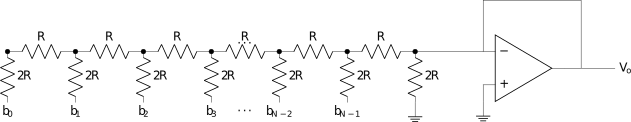
\includegraphics[width=0.8\linewidth, alt={Resistor ladder circuit diagram for a sample and hold system. The circuit has a horizontal row of six 2R resistors, each connected to a digital input labeled b0 through b3, bN2, and bN1. Below each 2R resistor is a corresponding R resistor, forming vertical pairs. The right end of the ladder connects to a voltage output labeled positive V-o.}]{figures/fig5_1.svg}
\end{figure}

then depending on the bit pattern at the output port $V$, the output of the buffer op-amp will be
\[
V_o = V_{ref}\frac{V}{2^N}
\]

If the port value is changed every sample time $T$, then the resister ladder and buffer op-amp combine to implement a zero-order hold circuit.

\subsection{Reconstruction(anti-imaging) filter}

The zero-order hold is followed by the reconstruction (anti-imaging) filter which low-pass filters the output and smooths-out the jumps from value to value.

With or without and anti-imaging filter the signal is positive. This can be followed by a summing amplifier to shoft the signal voltage up or down and amplify as needed.


\end{document}
